\documentclass[border=4pt]{standalone}
\usepackage[T1]{fontenc}
\usepackage{helvet}
\renewcommand{\familydefault}{\sfdefault}
\usepackage{graphicx}
\usepackage{caption}
\usepackage{amsmath}
\captionsetup{font={sf,footnotesize},labelfont={sf,bf,footnotesize},justification=justified,singlelinecheck=false}
\begin{document}
\setcounter{figure}{6}
\begin{minipage}{7.20in}
\centering
\begin{figure}[htbp]
    \centering
    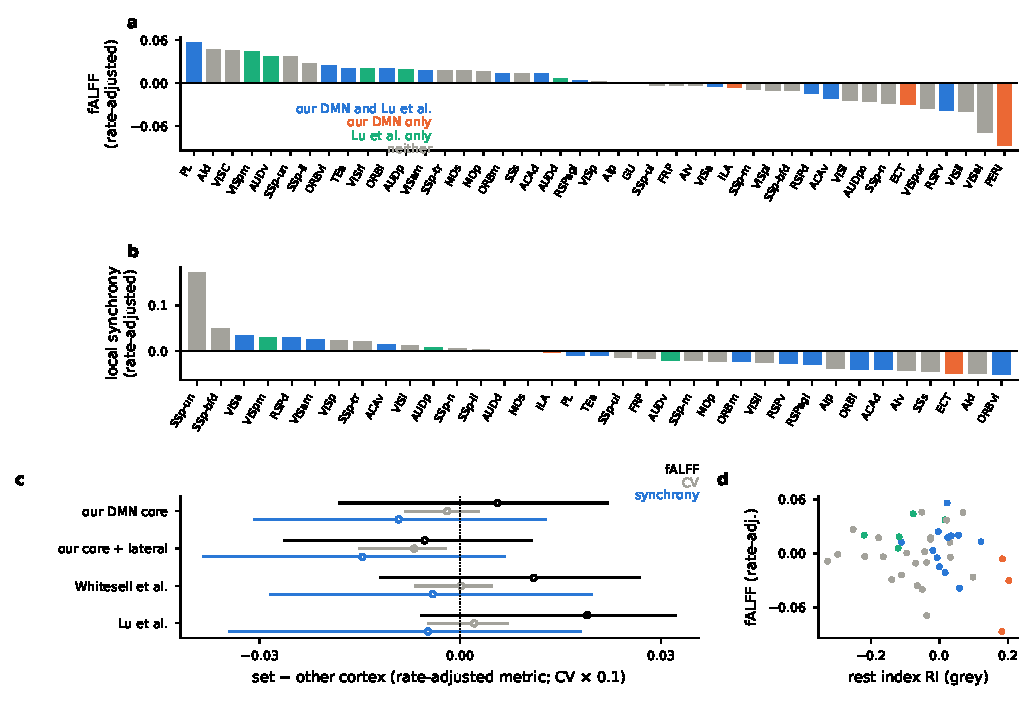
\includegraphics[width=\linewidth]{fig7_single_region_panels.pdf}
    \caption{\textbf{a} Single-region resting metrics need no co-recording, so they pool across animals (47,435 neurons, 396 sessions, 130 mice). fALFF per neuron: fraction of 0.01--0.1 Hz power in the 1 s binned rate over the whole grey-screen period after regressing wheel, licks and motion energy (the analogue of fMRI fALFF), residualised on log firing rate, averaged per cortical region. Colours as in Fig. 3. The map is reproducible across halves of the mice (Spearman--Brown 0.75) but DMN regions are spread throughout it. \textbf{b} Local synchrony (ReHo analogue): mean pairwise correlation between neurons of a region on one probe in still 1 s bins, residualised on rate (1,695 region-sessions, 116 mice). \textbf{c} Difference between each DMN definition and other cortex for fALFF, fluctuation amplitude (coefficient of variation, CV, scaled by 0.1) and local synchrony, all rate-adjusted: 95\% mouse-bootstrap CI; filled markers region-permutation p $<$ 0.05 (uncorrected). \textbf{d} Per region, grey-screen rest preference (RI, Fig. 3) against fALFF: Spearman $\rho$ = -0.05; the two single-region measures are unrelated.}
    \label{fig:grey_single}
\end{figure}
\end{minipage}
\end{document}
